\chapter{Bend Geometry in Liquid Crystals}
\label{ch:TwistBend}
\section{The structure of bend zeros}
\begin{figure}[htbp]
    \centering
    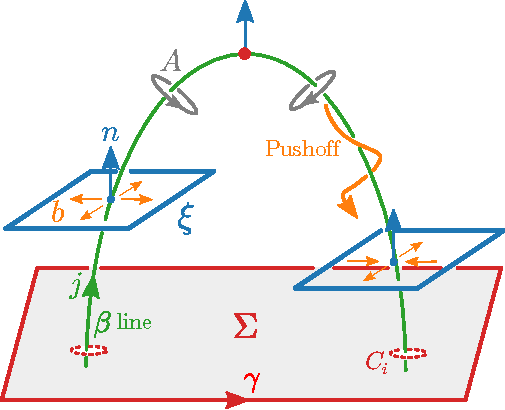
\includegraphics[keepaspectration, width=0.7\linewidth ]{\TwistBendFigures/BetaLine6.pdf}
    \caption{hi}
    \label{fig:BetaLines}
\end{figure}

Consider the un-normalised vector field dual to $A$, $\mathbf{B} := \langle b,b \rangle \langle A, \bullet \rangle$ --- the notation $\mathbf{B}$ is chosen to emphasise its similarity to the magnetic field around a current carrying wire. The vector $\mathbf{j} := \nabla \times \mathbf{B}$ points along the $\beta$ lines, orienting them according to the circulation of $A$ and $\mathbf{B}$, as shown in figure~\ref{fig:BetaLines} \cite{MachonThesis}. To see this, consider an orthonormal local trivialisation $(\w d_x, \w d_y,\bf n)$ in a tube around the $\beta$ line. Unlike $(\mathbf{b}, \mathbf{b}_\perp)$, both of which vanish on the $\beta$ line itself, $(\w d_x, \w d_y)$ are perfectly well defined and smooth, although at this stage they are not adapted to the $\beta$ line in any way. In such a trivialisation, ${\bf b} = b_x \w{d}_x + b_y \w{d}_y,\ {\bf b}_\perp = -b_x \w{d}_y + b_y \w{d}_x,\ \langle \w b, \w{b} \rangle = b_x^2 + b_y^2$. Expanding $A$ one finds
\begin{equation}
    A = \frac{b_x d b_y - b_y d b_x}{b_x^2 + b_y^2}+ \omega
    \label{eq:localA}
\end{equation}
where \omega := $\langle \w{d}_y, \nabla \w{d}_x \rangle$ is the connection $1$-form associated to $\nabla$ when using this local trivialisation. $(b_x,b_y,s)$, where $s$ is arclength along the $\beta$ line, form a local coordinate system with z-axis, given by $\nabla b_x \times \nabla b_y/|\nabla b_x \times \nabla b_y|$, tangent to the $\beta$ line\footnote{We assume that $(b_x, b_y)$ vanish linearly, so $\nabla b_x$ etc. is non-zero on the $\beta$ line and we have a well defined coordinate system.}. We may also define the associated cylindrical polar system $(\rho,\theta,z)$\footnote{Remember however that the associated cartesian vectors $\nabla b_x$ and $\nabla b_y$ are not orthonormal and so there is a Jacobian between this and a `true' polar system.}, in which $A = d\theta + \omega$; neglecting the smooth $\omega$ component, $A$ circulates as the azimuthal 1-form around the $\beta$ line (figure~\ref{fig:BetaLines}). Multiplying \eqref{eq:localA} through by $b_x^2 + b_y^2$ (which causes the $\omega$ term to vanish on the $\beta$ line) $\w{B} = b_x \nabla b_y - b_y \nabla b_x + (b_x^2 + b_y^2) \omega , \quad \w{j} = \nabla \times \w{B} =\nabla b_x \times \nabla b_y$. We emphasise that, as \eqref{eq:localA} shows, $A$ and $d\theta$ are well defined and continuous along the whole $\beta$ line.

\subsection{The local structure of bend zeros}
We may investigate the local structure of a $\beta$ line via a Taylor series in $\w b$ or, equivalently, by examining the structure of $\nabla \w b$ on the $\beta$ line --- for a generic $\beta$ line  this Taylor series is governed by linear terms, with corresponding  non-zero $\nabla \w b$. We have already seen that the director $\w n$ splits $T \mathbb{R}^3\approx L_n \oplus \xi$, with a corresponding splitting of $\nabla \w n$ into two pieces , $\nabla_\perp \w n $ and $\nabla_\parallel \w n$, in \S\ref{subsec:Geometry}, and one way to proceed is to do same to $\nabla \w b$. However, the $\beta$ line itself, in combination with $\w n$ along it, provides us with more structure than a single splitting --- it gives a canonical way to further split $\xi$, giving an adapated framing with which several other planes and splittings may then be defined. In figure \ref{fig:Splittings}(a) we show the $\beta$ line and $\w n$ at a g
eneric point, where $\w n$ and $\w j$ are neither parallel nor perpendicular. 
The normalised cross product $\w n \times \w j$ defines a vector $\w n_\lambda$ and orthogonal plane $\lambda$, and completing this triple in a right handed fashion defines a third vector $\w n_\chi$, with associated orthogonal plane $\chi$, the normalised projection of $\w j$ onto $\xi$. Setting $(\w d_x, \w d_y, \w n) = (\w n_\chi, \w n_\lambda, \w n)$ gives an adapted frame for the $\beta$ line, with the line itself always in the $\lambda$ plane. Note immeadiately that by construction, $\w n_\chi \cdot \w j \geq 0$, and further that this frame is undefined if $\w n \parallel \w j$. Across such points both $\w n_\chi$ and $\w n_\lambda$ change sign discontinuously, and the framing undergoes a $\pi$ rotation (as unoriented planes $\chi$ and $\lambda$ may be extended by continuity) --- this situtation is shown in figure  \ref{fig:Splittings}(b), and shall we return to it in a moment. As well as $\xi, \chi$ and $\lambda$, we also have the plane perpendicular to $\w j$ itself, given by $\mathrm{ker}(A)$. Loops in these planes measure winding about the $\beta$ line. We have two limiting cases, shown in figures \ref{fig:Splittings}(b) and (c). The first, as mentioned above, is shown in figure~\ref{fig:Splittings}(b), where $\w  n \parallel \w j$, $\xi = \mathrm{ker}(A)$ and a loop in $\chi$ intersects the $\beta$ line --- if we try to measure winding on this plane we encounter degenerate behaviour. In figure \ref{fig:Splittings}(c), $\w n \perp \w j$, $\chi = \mathrm{ker}(A)$ and a loop in $\xi$  intersects the $\beta$ line, likewise showing degenerate behviour. This latter case, where $\w n \cdot \w j= 0$, we refer to as a Legendrian point \citep{Geiges2009}. One notes that the degeneracy in figure \ref{fig:Splittings}(b) is of higher codimension than that in \ref{fig:Splittings}(c).
\begin{figure}[htbp]
    \centering
    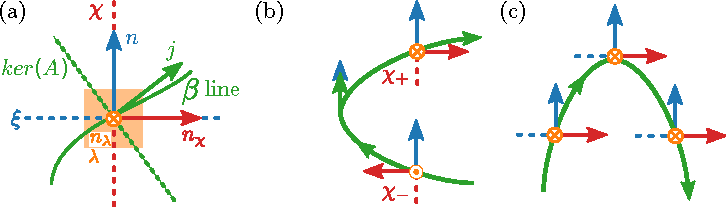
\includegraphics[keepaspectration, width=0.99\linewidth ]{\TwistBendFigures/Splittings.pdf}
    \caption{hi}
    \label{fig:Splittings}
\end{figure}

We now examine the structure of $\nabla \w b$ on the $\beta$ line, making use of the various planes defined above. Note first that, in general, $\nabla \w b \in T^*\mathbb{R}^3 \otimes T\mathbb{R}^3$, however on a $\beta$ line it lies in $T^*\mathbb{R}^3 \otimes \xi$, as $\w n \cdot \nabla \w b = - \w b \cdot \nabla \w n = 0$ on the $\beta$ line.  $\nabla \w b$ has the structure of a linear map $\mathbb{R}^3 \rightarrow \mathbb{R}^2$, with a one-dimensional kernel  which defines the $\beta$ line; $\w j$ lies in this kernel. We have that 
\begin{equation}
\w j = \mathrm{det}(\nabla^{\ker(A)}\w b) \hat{\w j} = \mathrm{det}(\nabla^\xi \w b) \w n + \mathrm{det}(\nabla^\chi \w b) \w n_\chi
\label{eq:IndexRelation}
\end{equation}
where $\nabla^\chi \w b$, for example, is the restriction of $\nabla \w b \in T^*\mathbb{R}^3 \otimes \xi $ to the space $\chi^* \otimes \xi$. Each equality in \eqref{eq:IndexRelation} is just a rewriting of the cross product $\nabla b_x \times \nabla b_y$, but they may be obtained directly by pulling back the volume form on $\xi$ via $\nabla \w b$. Using the second equality  in \eqref{eq:IndexRelation} as an example, we have the decomposition $\nabla \w b = \nabla^\xi \w b E_\xi + \nabla^\chi \w b E_\chi+ \nabla^\lambda \w b E_\lambda$, where $E_\bullet$ denotes projection onto the subspace $\bullet$. This decomposition carries through to the pullback, and since each of $\nabla^\xi \w b , \nabla^\chi \w b,\nabla^\lambda \w b $ is a map between vector spaces of the same dimension, the pullback simply scales the volume form by the determinant (up to a sign). Finally, by the construction of our framing, $\mathrm{det}(\nabla^\lambda \w b) =0$ --- if we were using an arbitrary framing all three terms would appear in \eqref{eq:IndexRelation}. Recall also that, by the construction of $\w n_\chi$, $\det\nabla^\chi \w b \geq 0$.

 \eqref{eq:IndexRelation} relates the windings we see in different measuring loops around the $\beta$ line, and allows us to examine winding behaviour as we pass through a Legendrian point. In the above discussion we focused on $\xi$ and $\chi$, but it is worth also describing what one observes when measuring winding on a general oriented plane $\gamma$. Pairing a unit vector in $\mathbb{R}^3$ to its orthogonal oriented plane, the space of all such planes is $S^2$, and we imagine $\w j $ defining a north pole. The set of all planes containing the $\beta$ line is then an equatorial circle which splits $S^2$ into two disconnected pieces --- in passing from one piece to another one encounters a plane containing the $\beta$ line, in which $\mathrm{det}(\nabla^\gamma \w b) = 0$ and across which $\mathrm{det}(\nabla^\gamma \w b) = 0$ changes sign. This description motivates the definition of an index $ I^\gamma_\beta := \mathrm{Sgn}(\mathrm{det}(\nabla^\gamma \w b)) =\mathrm{Sgn}(\w n_\gamma \cdot \w j)$, where $\w n_\gamma$ is the unit vector associated with the oriented plane $\gamma$. The most common measurement of this type is $I^\xi_\beta$ \citep{Nye1987,Berry1998,Berry2004}, which describes the winding of $\w b$ measured on a loop in the oriented plane $\xi$. The value of $I^\gamma_\beta$ depends on which of the two equivalence classes outlined above $\gamma$ belongs to; if it is degenerate and $\mathrm{det}(\nabla^\gamma \w b)=0$, we set $I^\gamma_\beta=0$. By construction, $I^\lambda_\beta=0$, $I^\chi_\beta= \{0,1\}$. This latter fact is a little subtle given the reversal of $\w n_\chi$ when $\w n \parallel \w j$; we return to it in a moment.  

 Let us now consider situations of degeneracy in order of codimension, beginning with a Legendrian point (figure  \ref{fig:Splittings}(c)). At the point itself $\w n \cdot \w j =0$ so $I^\xi_\beta=0$ and we encounter degenerate winding on $\xi$; across the point these quantities change sign. By contrast, the winding measured in $\mathrm{ker}(A) = \chi$, given by $I^{\chi}_\beta$, is perfectly well behaved. The dual situation occurs when $\w n \cdot \w j = \pm 1$, $I^\chi_\beta=0$ (figure \ref{fig:Splittings}(b)). Across such points, the orientation of $\chi$ reverses --- to be precise, let us define a $-$ and $+$ side of the point, with associated oriented planes, $\chi_-$ and $\chi_+$ which may be smoothly continued across the singular point and so defined on a neighborhood of it. On the $-$ side $I^\chi_\beta = I_\beta^{\chi_-}$ and on the $+$ side $I_{\beta}^\chi = I_{\beta}^{\chi_+}$. We have that $I_{\beta}^{\chi_+} = -I_{\beta}^{\chi_-}$, and so measurement of index on a consistently oriented plane across the singular point shows a sign reversal. Finally, in general $\mathrm{det}(\nabla^{\ker(A)}\w b)^2 = \mathrm{det}(\nabla^\xi \w b)^2+ \mathrm{det}(\nabla^\chi \w b)^2$, and so for $I^{\mathrm{ker}(A)}_\beta$ to change sign we require that $I^\xi_\beta = I^\chi_\beta = I^\lambda_\beta=0$, in other words that $\w j$ vanish, an even higher codimension degeneracy in which $\mathrm{ker}(\nabla \w b)$ become two dimensional and the coordinate system $(b_x,b_y)$ defined above breaks down. 

We briefly explore how these constructions appear when given a concrete, but arbitary, framing $(\w d_x,\w d_y,\w n)$.With respect to our framing $\nabla \w b$ is a $2\times3$ matrix and we have a Taylor series
\begin{align}
\begin{pmatrix}b_x \\ b_y\end{pmatrix} = 
\begin{pmatrix} 
    \nabla^\xi \w b_{xx} & \nabla^\xi \w b_{xy} & s_{xz}\\
    \nabla^\xi \w b_{yx} & \nabla^\xi \w b_{yy} & s_{yz}\\ 
\end{pmatrix}
\begin{pmatrix}x \\ y \\ z \end{pmatrix}  
+ O(2)
\label{eq:gradbmatrix}
\end{align}
where $s_{xz},s_{yz}$ are currently regarded simply as undetermined constants in the Taylor series. How should we extract the adapted frame, orientation of the $\beta$ line and local windings from this matrix? $I_\beta^\xi$ is immeadiate. $\w j$ is given by
\begin{align}
    \w j &= (\nabla^\xi \w b_{xy}s_{yz} - \nabla^\xi \w b_{yy}s_{xz})\w d_x -( \nabla^\xi \w b_{xx}s_{yz} - \nabla^\xi \w b_{yx}s_{xz})\w d_y + \mathrm{det}(\nabla^\xi \w b) \w n \\
         &= \mathrm{det}(\nabla^{\chi^{'}} \w b)\w d_x  -\mathrm{det}(\nabla^{\lambda^{'}} \w b)\w d_y + \mathrm{det}(\nabla^\xi \w b) \w n = \mathrm{det}(\nabla^{\chi}\w b)\w n_\chi + \mathrm{det}(\nabla^\xi \w b) \w n
\end{align}
where $\chi'$ and $\lambda'$ are the planes associated to the unadapted frame $(\w d_x,\w d_y, \w n)$. We have that $\mathrm{det}(\nabla^{\chi} \w b)= (\mathrm{det}(\nabla^{\lambda^{'}} \w b)^2 + \mathrm{det}(\nabla^{\chi'}\w b)^2)^\frac{1}{2}$, where we may safely choose the positive branch of the square root by construction of $n_\chi$. Away from a Legendrian point $\w{j}$ may also be written as $\w j = \mathrm{det}(\nabla^\xi \w b)(\nabla^\xi \w b^{-1}\w{s},1)^T$, where $\w s = (s_{xz}, s_{yz})^T$, and so the orientation oh the $\beta$ line is determined by $\nabla^\xi \w b^{-1} \w s$ --- specifically, its angle to the local z-axis is given by $\tan\theta = \mathrm{det}(\nabla^{\chi}\w b)/ \mathrm{det}(\nabla^{\xi}\w b)= \w s^T (\nabla^\xi \w b^{-1})^T \nabla^\xi \w b^{-1} \w s$, and to the $x$-axis by $\cos \phi =\mathrm{det}(\nabla^{\chi'}\w b) /\mathrm{det}(\nabla^{\chi}\w b)$ --- a rotation by $\phi$ adapts the framing, bringing $\chi'=\chi, \lambda' = \lambda$, at which point \eqref{eq:gradbmatrix} adopts the form
\begin{align}
\begin{pmatrix}b_x \\ b_y\end{pmatrix} = 
\begin{pmatrix} 
     \cot \theta s_{xz}& \nabla^\xi \w b_{xy} &s_{xz}\\
    \cot \theta s_{yz}& \nabla^\xi \w b_{yy} & s_{yz}\\ 
\end{pmatrix}
\begin{pmatrix}x \\ y \\ z \end{pmatrix}  
+O(2)
\label{eq:gradbmatrix}
\end{align}
where $\nabla^\xi \w b_{xy}$ etc. now refer to the rotated coordinate values. At a Legendrian point, $\mathrm{det}(\nabla^\xi \w b)=0$, but the above expressions still hold in the limit $\tan \theta \rightarrow \pi/2, \cot \theta \rightarrow 0$.
\subsection{Relating local bend structure to director gradients}

 We may relate the operators defined above to director derivatives: a direct calculation yields $\nabla^\xi \w{b} = (\nabla^\xi{\bf n})^2+\nabla^L \nabla^\xi{\bf n}$ , $\nabla^L \w b = (\nabla^L)^2 \w n$. $\nabla^{\xi}{\bf n}$ defines a linear transformation on the plane perpendicular to the director ($xy$-plane), and is called the shape operator of the director field~\cite{MachonThesis,AlexanderBook}. With respect to an arbitrary $(\w d_x,\w d_y, \w n)$ frame the corresponding Taylor series for the director, retaining only terms that contribute to the bend at linear order, is
\begin{align}
\begin{pmatrix} n_x \\ n_y \end{pmatrix} & = \biggl( \Bigl. \nabla^\xi {\bf n} \Bigr\rvert_0 + z \Bigl. \bigl( \nabla^L\nabla^\xi {\bf n} \bigr) \Bigr\rvert_0 \biggr) \begin{pmatrix} x \\ y \end{pmatrix} + \frac{1}{2} z^2 \begin{pmatrix} (\nabla^L)^2 n_x \\ (\nabla^L)^2 n_y \end{pmatrix}, \\
\end{align}
giving bend
\begin{align}
\begin{pmatrix}b_x \\ b_y\end{pmatrix} & =
 \biggl( \Big( \Bigl. \nabla^\xi {\bf n} \Bigr\rvert_0 \Big)^2 + \Bigl. \nabla^L\nabla^\xi {\bf n} \Bigr\rvert_0 \biggr) \begin{pmatrix} x \\ y \end{pmatrix}
 + z \begin{pmatrix}(\nabla^L)^2 n_x \\ (\nabla^L)^2 n_y \end{pmatrix}
\label{eq:LocalBend}
\end{align}
which may then be cast into the form of \eqref{eq:gradbmatrix}.

$\nabla^\xi \w{b}$ itself may be further decomposed into two components, a spin 0 component $\nabla^{\xi, +} \w{b}$ with positive determinant and winding and a spin 2 component $\nabla^{\xi, -} \w{b}$ with negative determinant and winding: $\nabla^\xi \w{b} = \nabla^{\xi,+} \w{b} + \nabla^{\xi,-} \w{b}$ \cite{MachonThesis}. With this decomposition one finds that $\w{n} \cdot \w{j} = \mathrm{det}(\nabla^\xi \w{b}) = |\mathrm{det}(\nabla^{\xi, +} \w{b})| - |\mathrm{det}(\nabla^{\xi, -} \w{b})|$. Each of these components may be expressed in terms of the director. To do so, we recall the splitting of the shape operator \eqref{eq:GradientDecompositionperp}
\begin{align}
    \nabla^\xi {\bf n}= \frac{\nabla \cdot {\bf n}}{2}I - \frac{{\bf n} \cdot \nabla \times {\bf n}}{2} J + \Delta
\end{align} 
which, with respect to our local $(\w d_1,\w d_2,\w n)$ basis, reads 
\begin{align}
 \nabla^\xi {\bf n}=\begin{pmatrix} s/2 + \Delta_1 & -q/2 + \Delta_2 \\ q/2 + \Delta_2 & s/2 - \Delta_1 \end{pmatrix} ,
\end{align} 
where $s = \nabla \cdot \w n$ is the splay, $q = \w n \cdot \nabla \times \w n$ is the twist and $\Delta_1$, $\Delta_2$ are the deviatoric components~\cite{MachonThesis,Selinger2019}. We find that
\begin{align}
\nabla^{\xi,+} \w{b} &=
\frac{1}{4}\Big(s^2 - q^2 + 4\Delta_1^2 + 4\Delta_2^2 +2\partial_z s\Big)I+
\frac{1}{2} \Big(sq + \partial_z q \Big)J  \\
\nabla^{\xi,-} \w{b} &= s \Delta +\partial_z \Delta.
\end{align}
 Note that in the absence of $z$ variation, $\nabla^\xi \w{b} = (\nabla^\xi{\bf n})^2$ and only an index of $I^\xi_\beta = +1$ as possible. The potential for negative winding is thus entirely contained within $\partial_z \Delta$. Explicitly, $\w{n} \cdot \w{j} = \mathrm{det}(\nabla^\xi \w{b}) = \left( (s/2)^2 +(q/2)^2 -\Delta_1^2 - \Delta_2^2\right)^2 +\left(s(q/2)^2 + \partial_z (q/2)\right)^2 - (\partial_z \Delta_1) ^2 - (\partial_z \Delta_2)^2 - s \partial_z(\Delta_1^2 + \Delta_2^2)$.  In figure \ref{fig:LocalProfiles} we show a variety of bend zeros with indices $I^\xi_\beta = \pm 1$ and their accompanying modes of director distortion.

\begin{figure}[htbp]
    \centering
    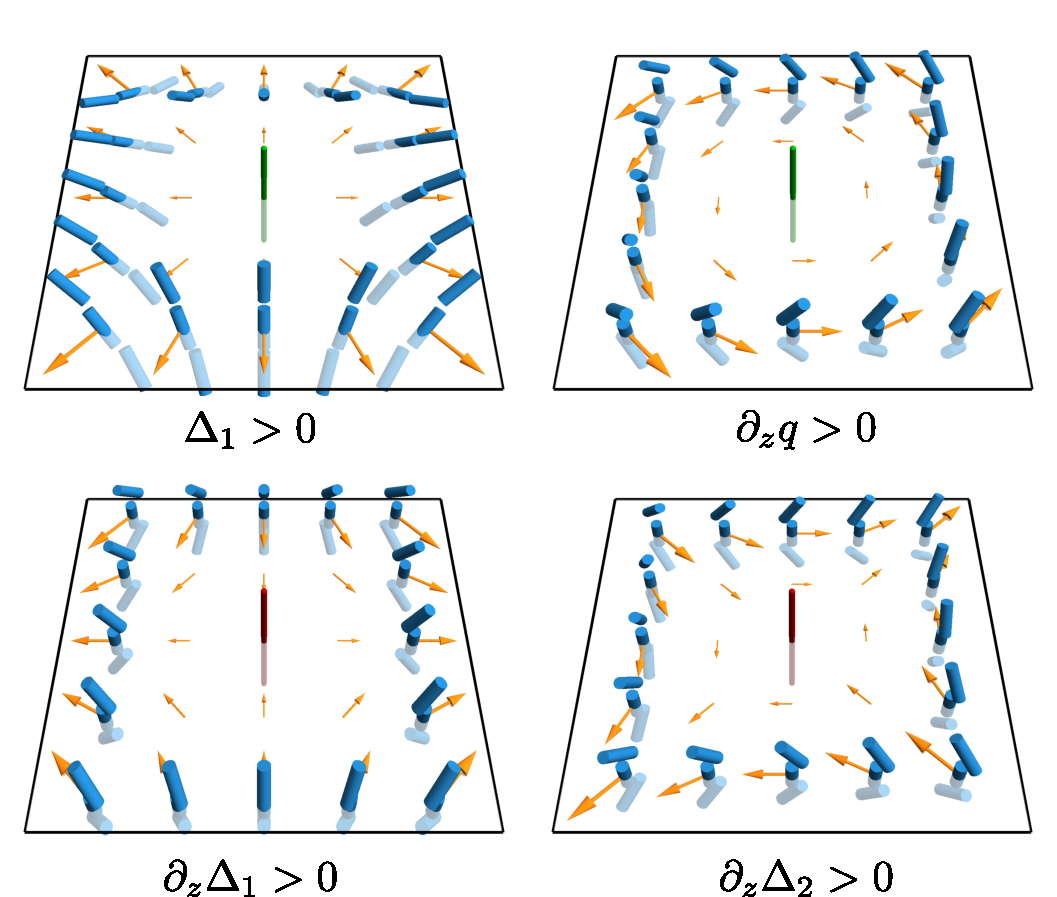
\includegraphics[keepaspectration, width=0.7\linewidth ]{\TwistBendFigures/LocalProfiles.pdf}
    \caption{Local profiles about $I_\beta = +1$ (green line) and $I_\beta = -1$ (red line) bend zeros, with director (blue cylinders) and bend vector (orange) shown in cross-section. Each panel shows the effect of a single parameter in  with the rest set to zero. $z$ variation in $\Delta$ is essential for a $I_\beta = -1$ zero.}
    \label{fig:LocalProfiles}
\end{figure}


\begin{comment}







\section{Topological Significance}

On the complement of the bend zeros, we define an orthonormal connection 1-form
\begin{equation}
    A = \langle \nabla \tilde{e}_1 ,\tilde{e}_2 \rangle = \frac{\langle \nabla e_1 ,e_2 \rangle}{\langle e_1,e_1 \rangle}  
\end{equation}

where $\tilde{e}_i$ is the normalised version of $e_i$. A few remarks about this definition are in order. Firstly, the connecction $\nabla$ at play here is a connection on the bundle $\xi$, and is globally well defined as the restriction of the ambient connection of manifold to the plane field. Equivalently, it is the pullback connection induced by the map ${\bf n}: M \rightarrow S^2$ --- this second formulation is good to remember. The sections $(e_1,e_2)$ are, however, only well defined on the complement of the bend zeros, and this carries through to $A$. 

Inserting a measuring surface $\Sigma$ with boundary $\gamma$ into $M$ one has a Gauss-Bonnet style result:
\begin{equation}
 \int_\gamma A - \int_\Sigma dA = \sum_i \int d \theta = \sum_i \mathrm{index}_\Sigma \beta_i
\end{equation}
The sum of these indices computes the degree of the map ${\bf n}:\Sigma \rightarrow S^2$, known as the skyrmion number. This is analogous to how the integration of the curvature form computes the degree of the Gauss map, and this again may be computed by summing the umbilic points of a surface. The number of $\beta$ lines facilitates this same count.

$A$, considered as a vector field $\bf A$, orients the umbilics , its curl giving a tangent vector, $\bf B = \nabla \times \bf A$. Thinking in terms of the magnetostatic potential and field around a wire, this is not overly surprising. One should weight the local profile around a $\beta$ line by the factor $\mathrm{Sgn}(\bf n \cdot B)$. The switches signs when the $\beta$ line is not transverse to the plane field $\xi$.


\end{comment}
